

The objective of the Client Side Application is to render a User Interface capable of interacting with a user,
enabling the collection of flight requests, and presentation of usefull solutions.
In order to be able to achieve this goals, the User Interface is built using the \textit{React}, 
the application state is managed through \textit{Redux},
and the responses for user requests are processed by a third-party API, the Server Side application.

Any application built using React and Redux evolves around a concept called \textit{State}.
The state of the application is stored inside the Redux Store, 
and it containts all the relevant data regarding the current available information, which, 
in this case, is summarized by the data collected from the user, and any data collected from third-party API's.
The complete state cycle of the developed application is summarized in figure \ref{fig:app_state_cycle}.

\begin{figure}[htpb]
  \centering
  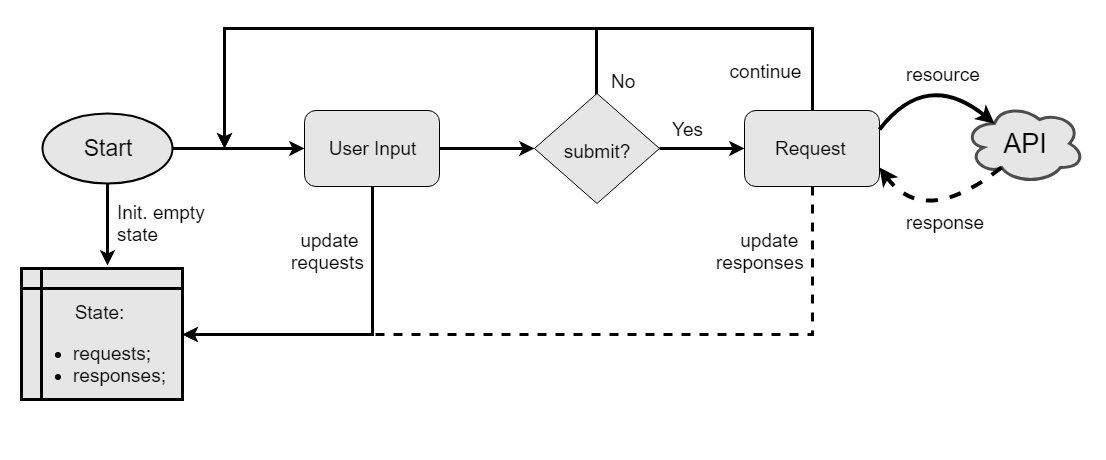
\includegraphics[width=\textwidth]{./Figures/system_implementation/state_flow.png}
  \caption{Block diagram of the state cycle of the Client Side Application.}
  \label{fig:app_state_cycle}  
\end{figure}


Although the user contributes indirectly to a state update, by, for example, filling or updating a certain form,
the state can only be modified by a class of functions called \textit{Reducers}.
Reducers are pure functions, which means that they always produce the same result for the same input.
Each time an action is dispatched, a reducer catches that action, and updates the state of the application.
This is usefull for many reasons. To give an example, consider the act of filling a form with the information 
regarding an airport. The user introduces may introduce a city name, but the reducer 
may complment this with more meaningfull data as, f.e., the airport ICAO code.  

The views of the User Interface are created by the React library,
based on the current state of the application and, each time the state is updated,
so is the UI. In order to have all views updates with the current state,
React proposes a top down hierarchy, divided into \textit{Containers} and \textit{Components}.
Containers are on the top of the hierarchy, and are directly connected to the redux store,
receiving the current state of the application. These containers usually
do not handle presentation logic themselves, but invoke components which do.
These components may receive parts of the state, \textit{props}, which may be relevant for rendering purposes,
as, for example, the already introduced input of a user form, or the response to a user request.

Although a React application is always up to date with the current state,
it does not re-render the entire page every time the state is updated. 
Instead, it compares the current DOM structure to a virtual DOM introduced by React,
and indentifies which components must be updated. This enables a fast and effective 
update of the User Interface.

Figure \ref{fig:react_redux_app} introduces the complete architecture of a React/Redux application, 
including some of the concepts previously discussed.
This figure illustrates the top down hierarchy, by having a single component in the top of the hierarchy,
which instantiates the store, and renders the complete application, by invoking the containers 
which are connected to the relevant presentiational components.
This figure also illustrates the interaction with the store, and with third-party API's.
Finnally, it is important to note that a browser can only render HTML,
and the entirety of the application is built using a javascript library. Thus, it is necessary 
to inject the created javascript with all the business and presentation logic, into the html file served 
to the user. This is usually achieved by using a package compiler called \textit{Webpack}, \textbf{cite}.

\begin{figure}[htpb]
  \centering
  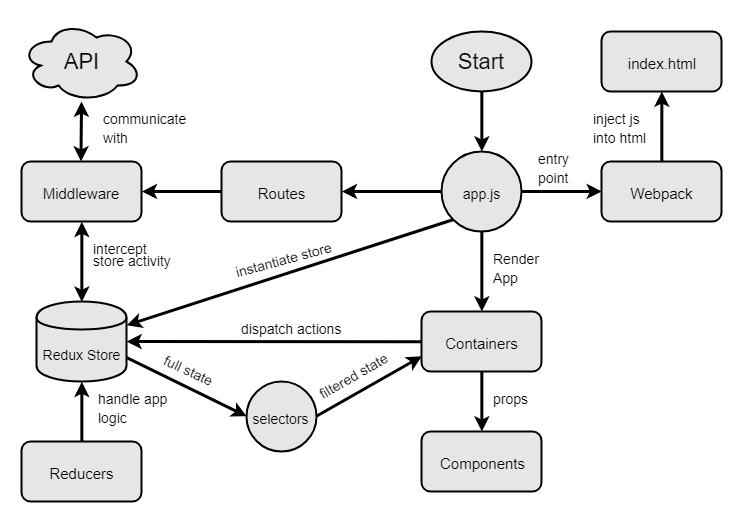
\includegraphics[width=\textwidth]{./Figures/system_implementation/react_redux_app.png}
  \caption{Building blocks of an application built using React And Redux}
  \label{fig:react_redux_app}  
\end{figure}




